% 必要な項目ができた場合は適宜サブセクションを追加してください
%\include{begin}

% イベント名を記入する
\section{朝食後の動き}

% 日時と場所を記入する
% 時刻は4桁で記入すること!

\subsection{日時・場所}
\begin{tabular}{p{2zw}rp{38zw}}
  日時 & : & 2019年4月6日(土) 08:30 $\sim$ 09:00\\
  場所 & : & 宿泊場所, 体育館
\end{tabular}

% 目的を記入する
\subsection{目的}
宿泊場所から体育館までの新入生の移動をスムーズに行い,イベント運営を円滑に行えるようにする.

\subsection{タイムスケジュール}
\begin{longtable}{p{3zw}p{39zw}}
   08:30 & \textbf{◎ 宿泊場所片付け} \\
         & \ \ \textbullet \ \ 食事を済ませたら各自宿泊場所に戻り,片付けが終わっていなければ片付けの続きを行う \\
         & \ \ \textbullet \ \ 宿泊場所から体育館への誘導スタッフは,新入生から棟の片付けが終わっていないと報告があった場合,朝食をとった後で宿泊場所に向かい,片付けの指示を行う(08:45まで)\\
         & \ \ \textbullet \ \ 日下,堀川は最後の人が出るまで食堂内で待機する \\
         & \ \ \textbullet \ \ 日下,堀川は食堂の片付けが終わり次第報告slackに連絡し,宿泊場所に戻る \\\\
  08:40 & \textbf{◎ プラカードの準備} \\
        & \ \ \textbullet \ \ 体育館でプラカードを持つスタッフ(塩谷,石野,角原,吉田,別役,横田,小松,藤沢,江川,中島,高橋(龍),新田,立岩,斎藤,小谷,生野)は,第一・二研修室に自分の荷物を置き,体育館へ行く \\
        %& \ \  \textbullet \ \ プラカードを持つスタッフは体育館で,図\ref{fig:nimotu2}に班の番号が書かれた紙を置く \\
        & \ \  \textbullet \ \ その後,19.5節の表に従って,各班のプラカードを持つ\\\\

  08:45 & \textbf{◎ 体育館に移動開始} \\
        & \ \ \textbullet \ \ 宿泊棟2階には戻れないため,残りのスタッフは荷物を全て持って宿泊棟1階へ降りる(その旨を同じ棟の新入生にも伝える) \\
        & \ \ \textbullet \ \ スタッフ・新入生共に,バスの号車ごとに分けて,荷物を第一・二研修室に置く \\
        & \ \ \textbullet \ \ 体育館に移動する前に,宿泊棟から体育館への誘導係(西森,藤田,別役,渡辺,高島,江川)は,新入生に体育館にしおりと筆記用具を持っていくように伝える \\
        & \ \ \textbullet \ \ 宿泊棟から体育館への誘導係(西森,藤田,別役,渡辺,高島,江川)は荷物を置いた新入生から順に誘導する \\
        %第一集会室でバスの号車ごとに各自荷物を置く\\
        & \ \ \textbullet \ \ その他のスタッフは付いていき,誘導の補助を行う \\
        & \ \ \textbullet \ \ 先生の誘導は,新入生の誘導後に行う \\
        %& \ \ \textbullet \ \ 体育館に到着したら誘導係は図14のようにおくよう新入生に指示を出す \\\\
        %& \ \ \textbullet \ \ 荷物を第一集会室に置いたらつどいの広間に移動する  \\\\

        &\textbf{◎ 体育館に移動開始(雨天時)}\\
        & \ \ \textbullet \ \ 上記の点に加えて新入生や先生に傘を出すことを促し,体育館の出入り口で傘を傘立てにいれるか,または壁にかける \\\\

  08:50 & \textbf{◎ 各班プラカード係待機} \\
        & \ \ \textbullet \ \ プラカードを持つスタッフはこの時間までに各班番号のプラカードを持ち,図\ref{fig:ice}に示した位置に待機しておく \\
        & \ \ \textbullet \ \ 誘導係の誘導の下,新入生が到着したら声掛けをしながら新入生を誘導し,グループの新入生が揃ったら円になって座らせる \\
        & \ \ \textbullet \ \ 食堂から新入生や先生方を誘導してきたスタッフは速やかに自分の班に移動する \\\\

  09:00 & \textbf{◎ 移動終了・イベント開始}  \\\\
\end{longtable}


% イベントに必要な役割と人数を記入する
% 担当者は決定次第追記する
% 記入例 ・司会者 2人(名前1、名前2)
\vspace{-3mm}
\subsection{人員配置}
\begin{itemize}
\item 食堂の片付け:日下,堀川
\item 宿泊棟から体育館への誘導係:西森,藤田,別役,渡辺,高島,江川
\item 体育館でプラカードを持つ係:塩谷,石野,角原,吉田,別役,横田,小松,藤沢,江川,中島,高橋(龍),新田,立岩,斎藤,小谷,生野
\end{itemize}

\subsection{各班プラカードとスタッフの対応}
\begin{table}[h]
\begin{center}
\label{sec:card}
\begin{tabular}{|c|c||c|c||c|c||c|c|}
\hline
{班}&{スタッフ}&{班}&{スタッフ}&{班}&{スタッフ}&{班}&{スタッフ} \\ \hline\hline
1 & 塩谷 & 5 & 別役 &  9 & 江川 & 13 & 立岩 \\ \hline
2 & 石野 & 6 & 横田 & 10 & 中島 & 14 & 斎藤 \\ \hline
3 & 角原 & 7 & 小松 & 11 & 高橋(龍) & 15 & 小谷 \\ \hline
4 & 吉田 & 8 & 藤沢 & 12 & 新田 &16 & 生野 \\ \hline
\end{tabular}
\end{center}
\end{table}

\vspace{-3mm}
\subsection{イベントの班分け}
%1班(真壁, 生野(イ)), 2班(石野, 小松), 3班(高島, 小野(生)), 4班(江川, 藤田(竜世)(イ)), 5班(別役, 明神), 6班(横井, 藤沢(ア), 横田(総)), 7班(東, 堀川(ア)), 8班(高橋(果), 立岩), 9班(小谷, 上村), 10班(日下, 藤田(竜貴)), 11班(角原, 野田), 12班(松尾, 以西(生)), 13班(平松, 渡辺), 14班(徳石, 岡本), 15班(高橋(錬), 長通(総)), 16班(南部, 宮尾)
\begin{figure}[H]
\begin{center}

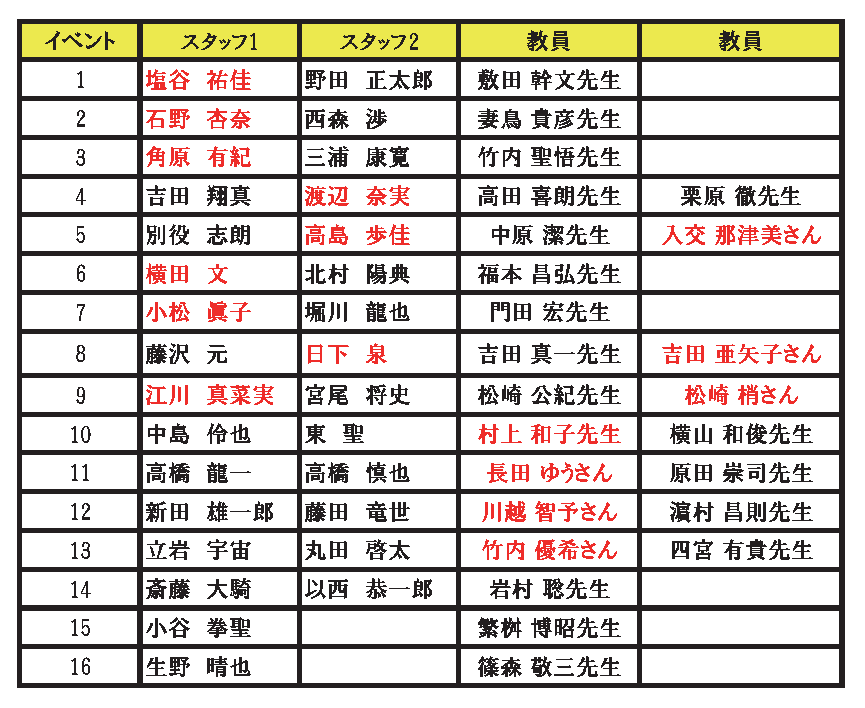
\includegraphics[scale=0.8]{./19/event_hanwake.eps}
\label{fig:Eventhanwake}
\caption{イベントの班分け図}
\end{center}
\end{figure}


%\subsection{備考}
%\begin{itemize}
%\end{itemize}

%\include{end}
